\documentclass[10pt]{article}
\usepackage[utf8]{inputenc}
\usepackage{geometry}
\usepackage{graphicx,graphics}
\usepackage{hyperref}
\usepackage{graphicx}
\usepackage{url}
\usepackage{float}
\usepackage{amsmath}
\usepackage{multicol}
\usepackage{amssymb}
\usepackage{multirow}
\usepackage{textcomp}
\usepackage{gensymb}
\usepackage{hhline}
\usepackage{array}
\usepackage{caption}
\usepackage{adjustbox}
\usepackage[spanish, es-tabla]{babel}
\usepackage[center]{titlesec}
\usepackage[table,xcdraw]{xcolor}

\geometry{top=2cm, bottom=2cm, left=1.5cm, right=1.5cm}
\spanishdecimal{,}
\setlength{\parskip}{0mm}

\renewcommand{\arraystretch}{1.3}
\renewcommand{\thesection}{\large\Roman{section}}
\renewcommand{\thesubsection}{\large\Alph{subsection}}

\providecommand{\abs}[1]{\lvert#1\rvert}
\title{
    Estudio de la constante de equilibrio y su relación con los reactivos y la temperatura
}
\author{
    \normalsize{
        \emph{Andrés F. Valencia Fonseca}$^{1}$,
        \emph{Nicolás Aguilera García}$^{2}$
    } \\
    \normalsize{
        \emph{Departamento de Física, Universidad del Valle, Cali, Colombia}
    } \\
    \small{$^{1}$2125166, $^{2}$21273030}
}
\date{(\small 8 de junio de 2023)}

\begin{document}
\maketitle

\begin{multicols*}{2}
    \section{\small ANÁLISIS Y RESULTADOS}

    \subsection*{\small \raggedright Resultados}

    Al realizar el laboratorio virtual se obtuvieron los siguientes resultados:

    \begin{table}[H]
        \centering
        \caption{Datos de comportamiento de la constante de equilibrio con respecto a la concentración inicial de los reactivos}
        \begin{adjustbox}{width=0.48\textwidth}
            \begin{tabular}{|c|c|c|c|c|c|}
                \hline
                \textbf{[SCN$^-$]i (M)} & \textbf{[Fe$^{3+}$]i (M)} & \textbf{[FeSCN$^{2+}$]e (M)} & \textbf{[SCN$^-$]e (M)} & \textbf{[Fe$^{3+}$]e (M)} & \textbf{Kc} \\
                \hline
                0.01                    & 0.01                      & 0.0055                       & 0.0045                  & 0.0045                    & 271.6       \\
                0.02                    & 0.01                      & 0.008                        & 0.012                   & 0.002                     & 333.3       \\
                0.03                    & 0.01                      & 0.009                        & 0.021                   & 0.001                     & 428.5       \\
                0.04                    & 0.01                      & 0.095                        & -0.055                  & -0.085                    & 20.3        \\
                0.05                    & 0.01                      & 0.009                        & 0.041                   & 0.001                     & 219.5       \\
                0.02                    & 0.01                      & 0.008                        & 0.012                   & 0.002                     & 333.3       \\
                0.02                    & 0.02                      & 0.0125                       & 0.0075                  & 0.0075                    & 222.2       \\
                0.02                    & 0.03                      & 0.0145                       & 0.0055                  & 0.0155                    & 170.0       \\
                \hline
            \end{tabular}
        \end{adjustbox}
    \end{table}

    \begin{table}[H]
        \centering
        \caption{Datos de comportamiento de la constante de equilibrio con respecto a la temperatura}
        \begin{adjustbox}{width=0.48\textwidth}
            \begin{tabular}{|c|c|c|c|c|}
                \hline
                \textbf{T (ºC)} & \textbf{[FeSCN$^{2+}$]e (M)} & \textbf{[SCN$^-$]e (M)} & \textbf{[Fe$^{3+}$]e (M)} & \textbf{Kc} \\
                \hline
                5               & 0.0140                       & 0.006                   & 0.006                     & 388.8       \\
                15              & 0.0135                       & 0.0065                  & 0.0065                    & 319.5       \\
                30              & 0.0120                       & 0.008                   & 0.008                     & 187.5       \\
                40              & 0.0115                       & 0.0085                  & 0.0085                    & 159.1       \\
                60              & 0.0100                       & 0.01                    & 0.01                      & 100.0       \\
                80              & 0.0085                       & 0.0115                  & 0.0115                    & 64.2        \\
                \hline
            \end{tabular}
        \end{adjustbox}
    \end{table}

    \subsection*{\small \raggedright Análisis}

    Observando el comportamiento de los valores de $K_c$ cuando se varian las concentraciones iniciales, se puede ver que a medida que aumenta la concentración inicial de los reactivos, la constante de equilibrio aumenta. Lo cual concuerda con lo que dicta el principio de Le Chatelier.

    Por otro lado, al observar el comportamiento de los valores de $K_c$ cuando se varia la temperatura, se puede ver que a medida que aumenta la temperatura, la constante de equilibrio disminuye, con un comportamiento casi lineal que puede ser observado en la grafica:

    \begin{figure}[H]
        \centering
        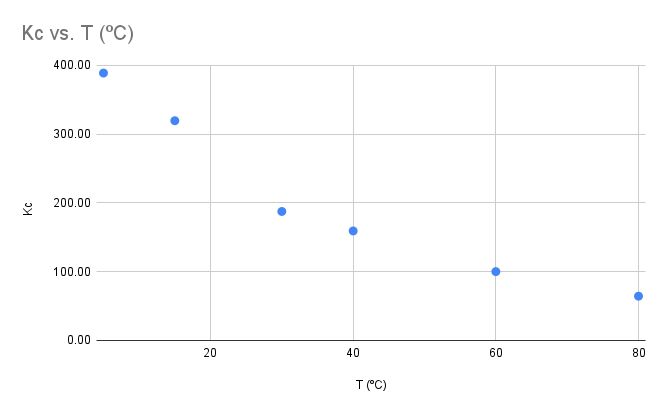
\includegraphics[scale=0.38]{./img/tcvskc.png}
        \caption{Comportamiento de la constante de equilibrio con respecto a la temperatura}
        \label{datos1}
    \end{figure}

    \subsection*{\small \raggedright ¿Cómo varía la constante de equilibrio con las concentraciones de los reactivos?}

    La constante de equilibrio ($K_c$) es una medida de la relación entre las concentraciones de los productos y los reactivos en una reacción química en equilibrio. La variación de la constante de equilibrio con las concentraciones de los reactivos se rige por el principio de Le Chatelier. Según este principio, si aumenta la concentración de los reactivos, el equilibrio se desplazará hacia la formación de productos para contrarrestar ese aumento. Como resultado, la constante de equilibrio aumentará. Por el contrario, si disminuye la concentración de los reactivos, el equilibrio se desplazará hacia la formación de reactivos y la constante de equilibrio disminuirá.

    \subsection*{\small \raggedright ¿Cómo varía la constante de equilibrio con la temperatura?}

    La constante de equilibrio ($K_c$) también puede variar con la temperatura. En general, un aumento de temperatura favorece una reacción endotérmica (absorbe calor) y desfavorece una reacción exotérmica (libera calor). Si una reacción es exotérmica, el aumento de temperatura disminuirá la constante de equilibrio, y si es endotérmica, el aumento de temperatura aumentará la constante de equilibrio. Esto se debe a que el aumento de temperatura proporciona energía adicional para romper o formar enlaces en la reacción, y el sistema se ajustará para contrarrestar ese cambio en energía.

    \subsection*{\small \raggedright El proceso de formación del ion complejo, ¿Es un proceso exotérmico o endotérmico?}

    El proceso de formación de un ion complejo puede ser tanto exotérmico como endotérmico, dependiendo de la reacción específica. En general, la formación de un ion complejo implica la interacción de un ion metálico con una especie o ligando que tiene electrones disponibles para formar enlaces coordinados. Durante esta interacción, se establecen enlaces coordinados entre el ion metálico y el ligando, lo que implica una redistribución de energía.

    Si la formación del ion complejo libera energía, es decir, si la energía de los enlaces formados es mayor que la energía de los enlaces rotos, entonces el proceso es exotérmico. En cambio, si la formación del ion complejo requiere energía adicional, es decir, si la energía de los enlaces rotos es mayor que la energía de los enlaces formados, entonces el proceso es endotérmico.

    La determinación exacta de si un proceso de formación de ion complejo es exotérmico o endotérmico dependerá de los valores específicos de energía asociados con las especies involucradas y puede variar de una reacción a otra.

    \section{\small CONCLUSIONES}

    
    Mediante este laboratorio se logró cumplir los objetivos planteados de determinar experimentalmente (mediante laboratorio virtual) el valor de la constante de equilibrio y visualizar su dependencia con la temperatura. Los resultados obtenidos respaldan los principios del equilibrio químico y el principio de Le Chatelier, ya que se observó que la constante de equilibrio aumenta al incrementar la concentración inicial de los reactivos, lo cual es coherente con el desplazamiento del equilibrio hacia la formación de productos. Asimismo, se comprobó que a medida que aumenta la temperatura, la constante de equilibrio disminuye, evidenciando el efecto de la energía adicional proporcionada en la formación o ruptura de enlaces.

\end{multicols*}
\end{document}